%==================================================================
% Ini adalah bab 2
% Silahkan edit sesuai kebutuhan, baik menambah atau mengurangi \section, \subsection
%==================================================================

\chapter[RENCANA KEGIATAN PRAKTIK INDUSTRI]{\\ RENCANA KEGIATAN PRAKTIK INDUSTRI}

\section{Profil Perusahaan \perusahaan}
Bagian ini digunakan apabila dibutuhkan, silahkan bisa ditambah atau dikurangi sesuai kebutuhan.

\subsection{Sub Dasar Teori 2.1.1}
Bagian ini digunakan apabila dibutuhkan, silahkan bisa ditambah atau dikurangi sesuai kebutuhan.

\section{Bentuk Kegiatan}
Bagian ini digunakan apabila dibutuhkan, silahkan bisa ditambah atau dikurangi sesuai kebutuhan.

\subsection{Subsection 3.1.1}
Bagian ini digunakan apabila dibutuhkan, silahkan bisa ditambah atau dikurangi sesuai kebutuhan.

\subsection{Subsection 3.1.2}
Bagian ini digunakan apabila dibutuhkan, silahkan bisa ditambah atau dikurangi sesuai kebutuhan.

\section{Tempat Pelaksanaan}
Bagian ini digunakan apabila dibutuhkan, silahkan bisa ditambah atau dikurangi sesuai kebutuhan.

\section{Jadwal dan Rencana Kegiatan}
Bagian ini digunakan apabila dibutuhkan, silahkan bisa ditambah atau dikurangi sesuai kebutuhan.

\section{Penulisan dengan \LaTeX}
Bagian ini menyediakan tutorial singkat mengenai beberapa lingkungan penulisan dasar yang sering digunakan dalam dokumen LaTeX. Penjelasan ini bertujuan untuk mempermudah pengguna dalam menulis dan mengatur dokumen dengan lebih efisien. Setiap bagian akan disertai contoh kode dan hasilnya untuk membantu pemahaman.

\subsection{List atau Daftar dengan \texttt{packed\_enum}}
Lingkungan \texttt{packed\_enum} digunakan untuk membuat daftar bernomor dengan jarak yang lebih rapat antar item. Ini sangat berguna untuk menampilkan langkah atau tahapan yang memiliki urutan. Berikut adalah contoh penggunaannya:

\begin{lstlisting}
    \begin{packed_enum}
        \item Langkah pertama adalah mengidentifikasi masalah yang ingin diselesaikan.
        \item Langkah kedua melibatkan analisis kebutuhan.
        \item Langkah ketiga adalah mengembangkan ide dan solusi alternatif.
        \item Langkah keempat adalah melakukan pengujian awal untuk mengevaluasi performa.
    \end{packed_enum}
\end{lstlisting}
    
Hasilnya akan tampak seperti berikut:
\begin{packed_enum}
    \item Langkah pertama adalah mengidentifikasi masalah yang ingin diselesaikan.
    \item Langkah kedua melibatkan analisis kebutuhan.
    \item Langkah ketiga adalah mengembangkan ide dan solusi alternatif.
    \item Langkah keempat adalah melakukan pengujian awal untuk mengevaluasi performa.
\end{packed_enum}

\subsection{List atau Daftar dengan \texttt{packed\_item}}
Lingkungan \texttt{packed\_item} digunakan untuk membuat daftar berpoin dengan jarak antar item yang lebih rapat, cocok untuk poin-poin yang tidak memerlukan urutan tertentu. Berikut adalah contoh penggunaannya:

\begin{lstlisting}
    \begin{packed_item}
        \item Meningkatkan kualitas sensor untuk akurasi yang lebih baik.
        \item Menambahkan modul komunikasi untuk kontrol jarak jauh.
        \item Mengoptimalkan kode untuk efisiensi.
        \item Menambah fitur penghematan energi.
    \end{packed_item}
\end{lstlisting}

Hasilnya akan tampak seperti berikut:
\begin{packed_item}
    \item Meningkatkan kualitas sensor untuk akurasi yang lebih baik.
    \item Menambahkan modul komunikasi untuk kontrol jarak jauh.
    \item Mengoptimalkan kode untuk efisiensi.
    \item Menambah fitur penghematan energi.
\end{packed_item}

\subsection{Menuliskan Kode dengan Listing}
Lingkungan \texttt{lstlisting} memungkinkan kita untuk menuliskan atau menyisipkan kode Python, C++, Arduino, Java atau lainnya dalam dokumen LaTeX dengan format yang rapi dan terstruktur. Pada bagian ini, kita akan melihat dua cara untuk menuliskan kode Python: secara langsung di dalam dokumen dan dengan mengambil dari file eksternal.

\Cref{lst:python_direct} menunjukkan fungsi Python yang menghitung faktorial dari sebuah angka. Kode ini ditulis langsung di dalam dokumen LaTeX menggunakan lingkungan \texttt{lstlisting} dengan format diawali dengan \texttt{\textbackslash begin\{lstlisting\}[language=Python, caption=Contoh Kode Python Langsung, label=lst:python\_direct]} dan diakhiri dengan \texttt{\textbackslash end\{lstlisting\}}, dimana:
\begin{packed_item}
    \item \texttt{language=Python}: Mengatur pewarnaan sintaksis untuk Python.
    \item \texttt{caption}: Menambahkan keterangan di atas kode untuk menjelaskan isi kode.
    \item \texttt{label}: Menambahkan label untuk memudahkan referensi kode dalam dokumen.
\end{packed_item}

\begin{lstlisting}[language=Python, caption=Contoh Kode Python Langsung, label=lst:python_direct]
    def factorial(n):
        if n == 0:
            return 1
        else:
            return n * factorial(n-1)
\end{lstlisting}

Jika Anda memiliki file kode Python di folder tertentu (misalnya, di \texttt{kode/code\_sample.py}), Anda bisa menyisipkan kode tersebut langsung ke dalam dokumen LaTeX menggunakan perintah \texttt{\textbackslash lstinputlisting}. Berikut \cref{lst:python_file} dengan format penulisan \texttt{\textbackslash lstinputlisting[language=Python, caption=Contoh Kode Python dari File, label=lst:python\_file]\{kode/code\_sample.py\}}, dimana:
\begin{packed_item}
    \item \texttt{language=Python}: Mengatur pewarnaan sintaksis untuk Python.
    \item \texttt{caption}: Menambahkan keterangan untuk kode yang diambil dari file.
    \item \texttt{label}: Menambahkan label untuk referensi.
    \item \texttt{\{kode/code\_sample.py\}}: Menentukan path atau lokasi file Python yang akan disisipkan. Pastikan file berada di dalam folder \texttt{kode} atau path yang sesuai.
\end{packed_item}

\lstinputlisting[language=Python, caption=Contoh Kode Python dari File, label=lst:python_file]{kode/code_sample.py}

\subsection{Menambahkan Gambar}
Untuk menambahkan gambar hal yang harus dilakukan adalah:
\begin{packed_enum}
    \item Menyalin file gambar (dalam format jpg \/ png) ke dalam folder \textit{gambar}
    \item Mengganti nama file dari gambar agar mudah dikenali, jangan diberi nama gambar-1,-2, dst
    \item Memasukkan seperti \cref{lst:kode_gambar}
\end{packed_enum}

\begin{lstlisting}[language=TeX, caption=Kode untuk Menyisipkan Gambar dalam Dokumen, label=lst:kode_gambar]
    \begin{figure}[H]
        \centering
        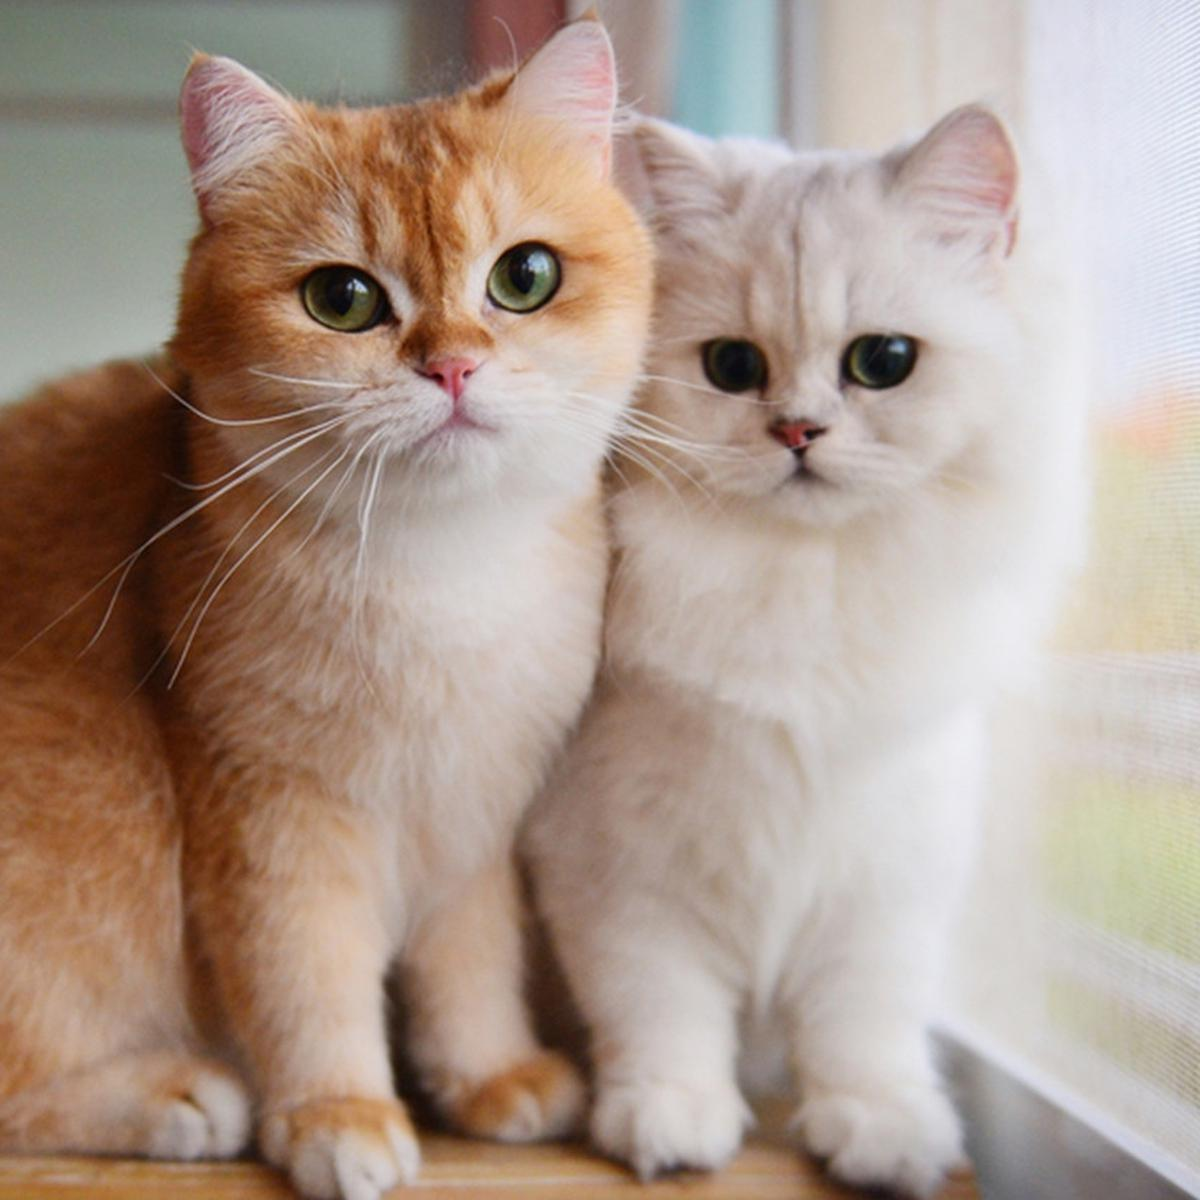
\includegraphics[scale=0.2]{gambar-kucing.jpg}
        \caption{Gambar Kucing Lucu dan Imut}
        \label{fig:kucing}
    \end{figure}
\end{lstlisting}

\noindent Berikut adalah penjelasan dari setiap baris pada kode di atas:

\begin{packed_enum}
    \item \texttt{\textbackslash begin\{figure\}[H] ... \textbackslash end\{figure\}}: Membuat lingkungan \texttt{figure} untuk menyisipkan gambar. Parameter \texttt{[H]} digunakan agar gambar diletakkan tepat di posisi yang ditentukan dalam kode. Opsi \textit{H} dapat diganti dengan \textit{h, t, b, p} sesuai kebutuhan.
    \item \texttt{\textbackslash centering}: Mengatur gambar agar berada di tengah halaman.
    \item \texttt{\textbackslash includegraphics[scale=0.2]\{gambar-kucing.jpg\}}: Memasukkan gambar dengan nama file \texttt{gambar-kucing.jpg}. Parameter \texttt{scale=0.2} mengatur ukuran gambar pada 20\% dari ukuran aslinya. Ubah nilainya untuk memperbesar atau memperkecil gambar.
    \item \texttt{\textbackslash caption\{Gambar Kucing Lucu dan Imut\}}: Menambahkan keterangan (caption) di bawah gambar yang akan muncul di Daftar Gambar dan disertai nomor gambar secara otomatis.
    \item \texttt{\textbackslash label\{fig:kucing\}}: Memberikan label pada gambar untuk merujuk gambar ini dalam teks menggunakan \texttt{\textbackslash cref\{fig:kucing\}} atau \texttt{\textbackslash ref\{fig:kucing\}} yang menghasilkan "Gambar 1" atau penomoran gambar sesuai urutan.
\end{packed_enum}

Hasilnya adalah terlihat seperti pada \cref{fig:kucing}.

\begin{figure}[H]
    \centering
    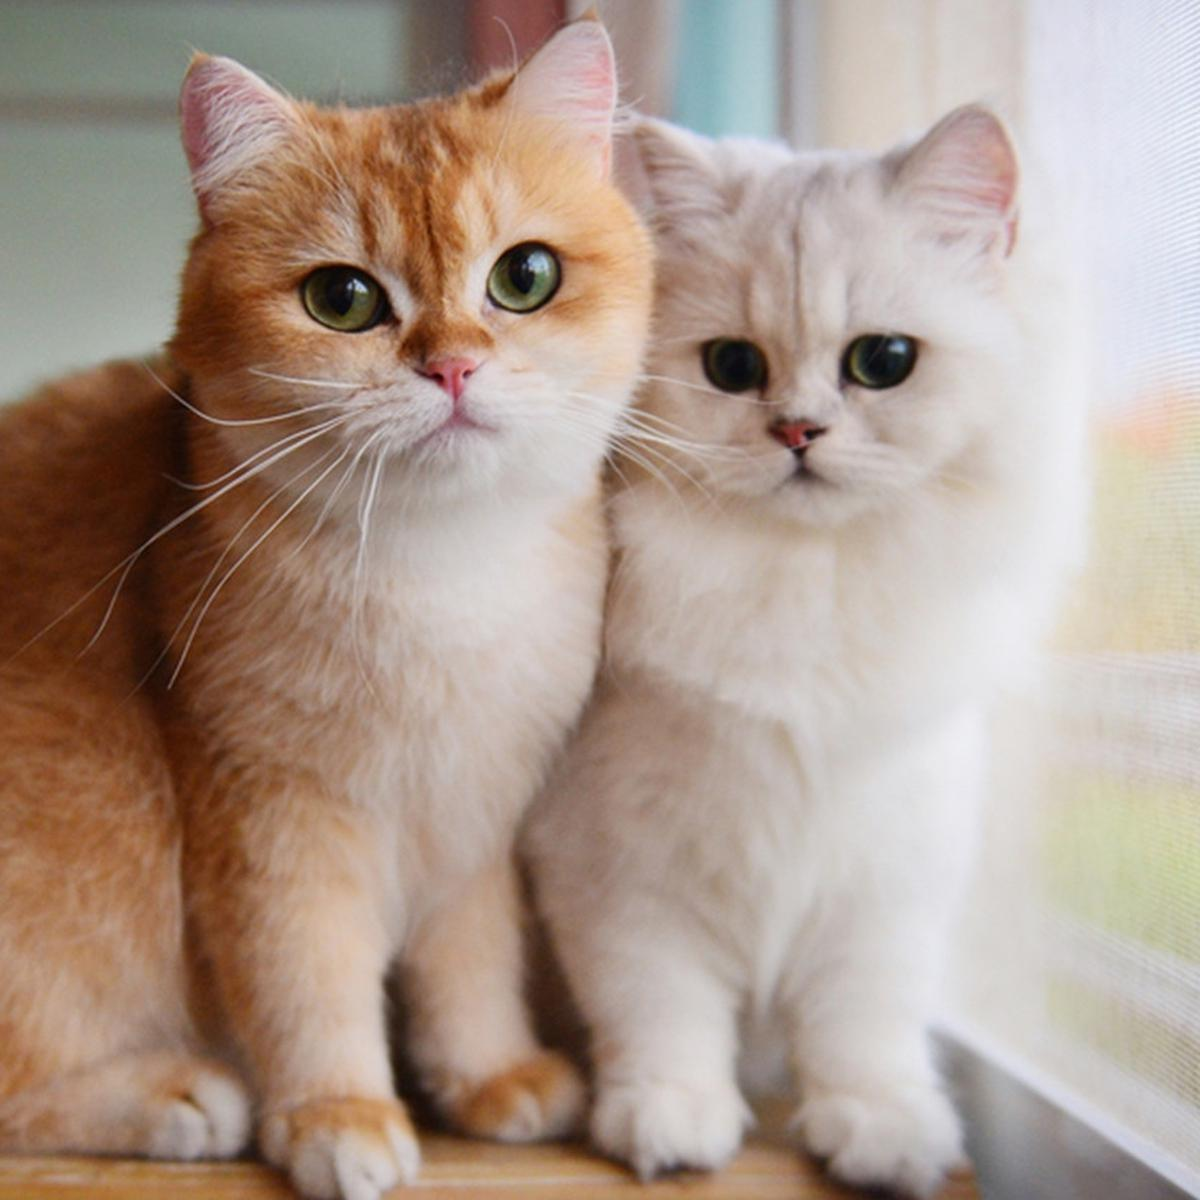
\includegraphics[scale=0.1]{gambar-kucing}
    \caption{Gambar Kucing Lucu dan Imut dengan scala 0.1}
    \label{fig:kucing}
\end{figure}

Setiap gambar harus dimention atau disebutkan didalam bacaan seperti berikut ini \cref{fig:kucing} dan \cref{fig:logoUNY}.

\begin{figure}[H]
    \centering
    
\includegraphics[scale=0.4]{logo-uny}
    \caption{Logo UNY dengan scala 0.4}
    \label{fig:logoUNY}
\end{figure}

Untuk menyisipkan beberapa gambar dalam satu kelompok dan satu caption utama, kita dapat menggunakan lingkungan \texttt{subfigure} di dalam lingkungan \texttt{figure}. Metode ini sangat bermanfaat jika kita ingin menyusun beberapa gambar berukuran kecil dalam satu baris atau kolom, dengan setiap gambar diberi caption masing-masing dan satu caption utama untuk keseluruhan gambar.

Kode berikut menunjukkan cara menyusun tiga gambar secara berdampingan dengan satu caption utama.

\begin{lstlisting}[language=TeX, caption=Kode untuk Menyisipkan Gambar dalam Dokumen dengan Subfigure, label=lst:kode_gambar_multi]
    \begin{figure}
        \centering
        \begin{subfigure}[b]{0.3\textwidth}
            \centering
            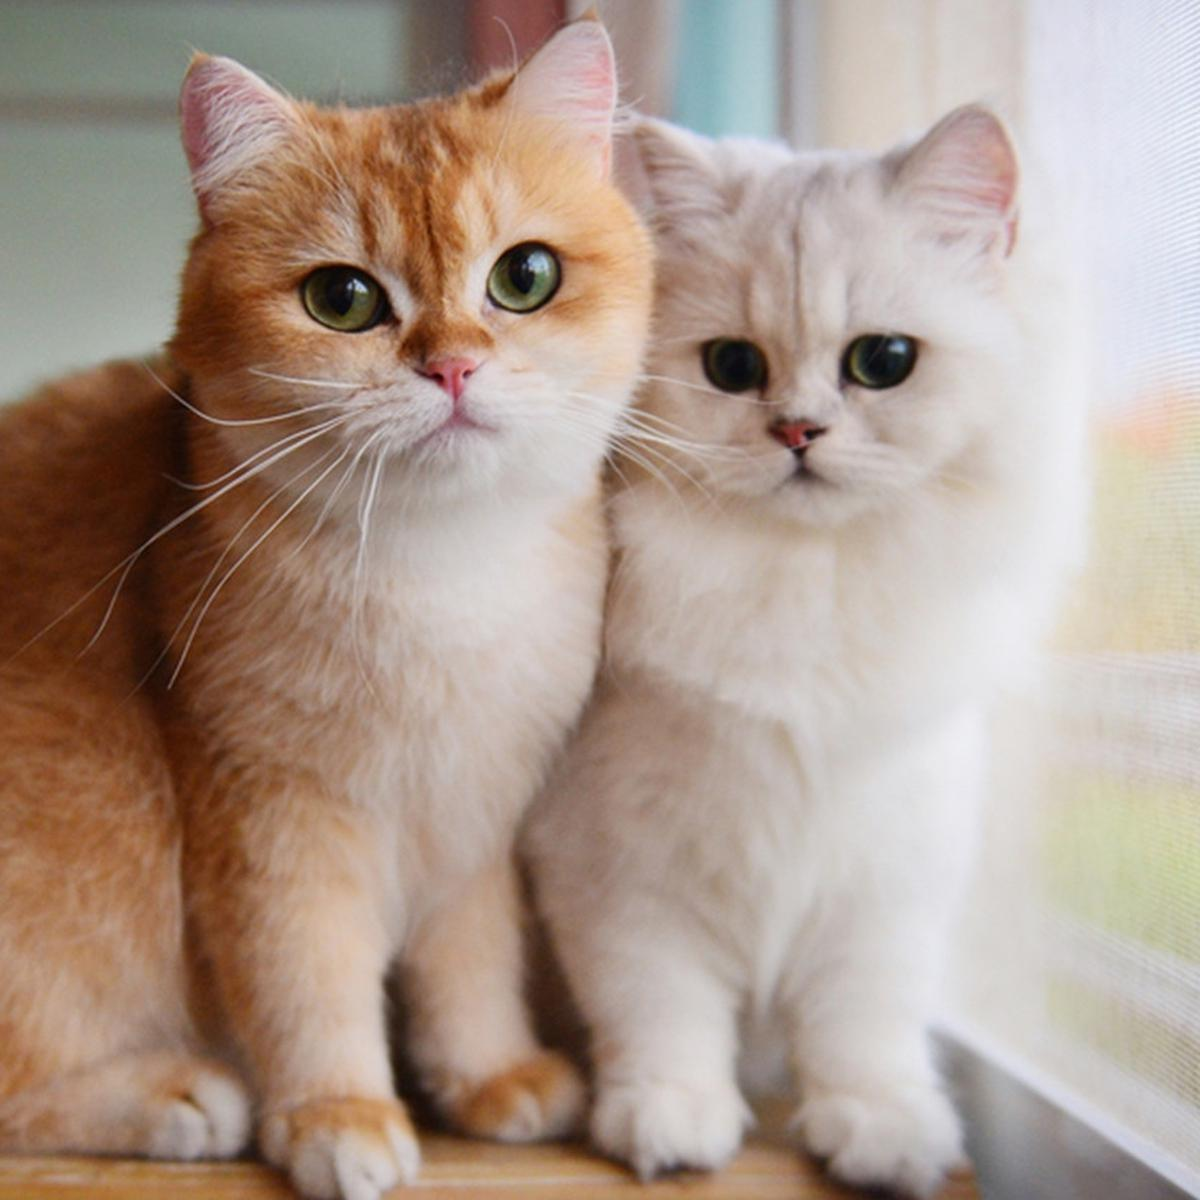
\includegraphics[width=\linewidth]{gambar-kucing.jpg}
            \caption{Kucing Lucu 1}
            \label{fig:kucing-a}
        \end{subfigure}
        \hfill
        \begin{subfigure}[b]{0.3\textwidth}
            \centering
            
\includegraphics[width=\linewidth]{logo-uny.png}
            \caption{Logo UNY}
            \label{fig:logo-uny-b}
        \end{subfigure}
        \hfill
        \begin{subfigure}[b]{0.3\textwidth}
            \centering
            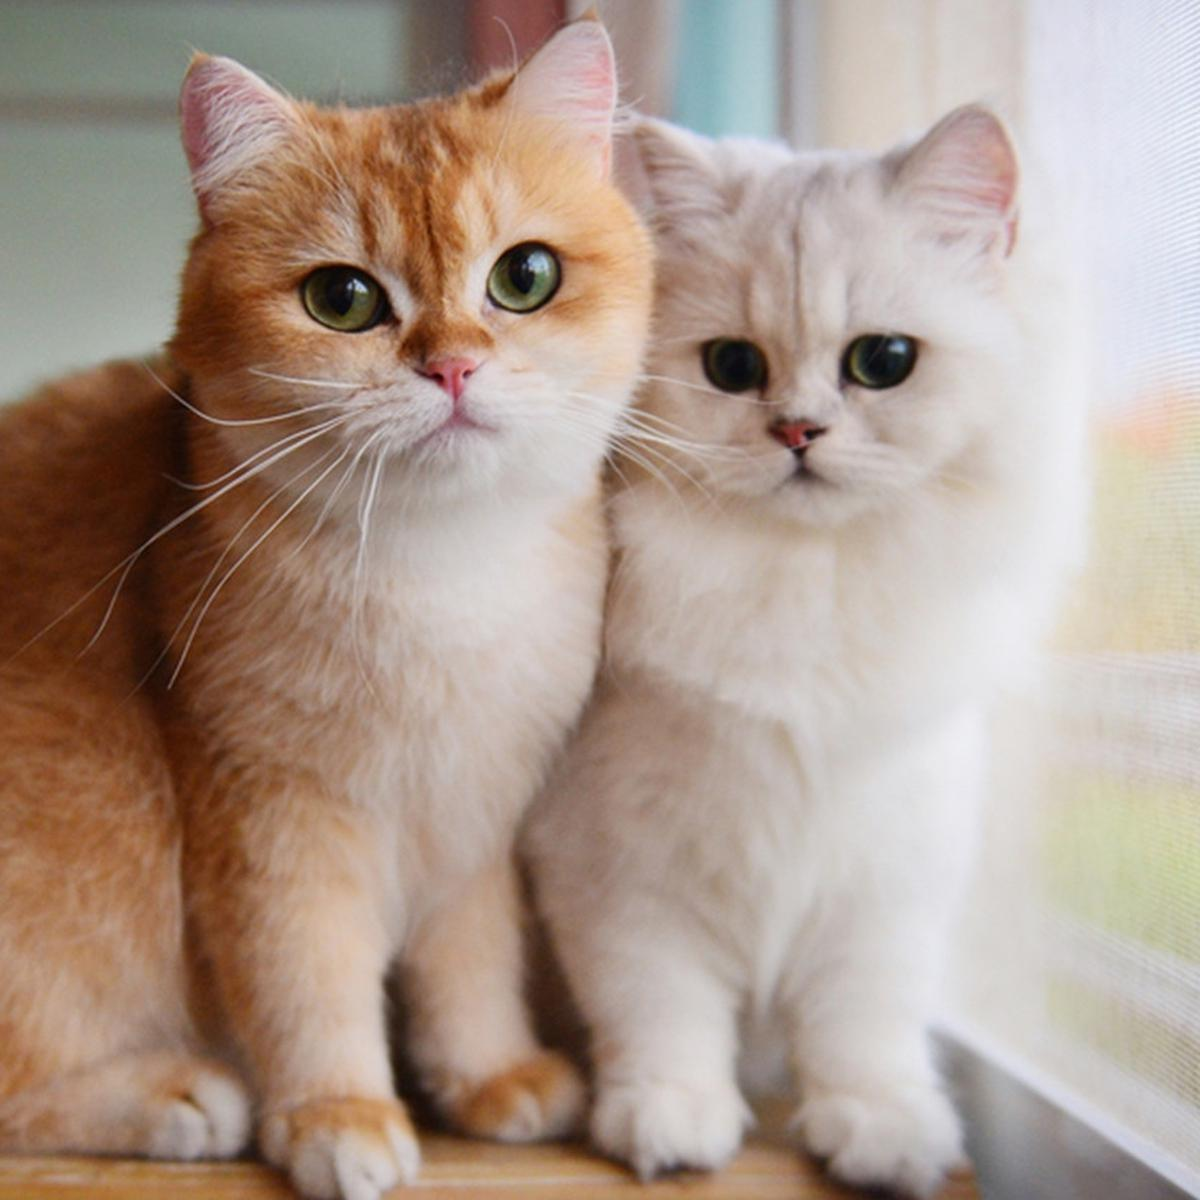
\includegraphics[width=\linewidth]{gambar-kucing.jpg}
            \caption{Kucing Lucu 2}
            \label{fig:kucing-c}
        \end{subfigure}
        \caption{Beberapa gambar yang disusun menjadi 1 bagian dengan penomoran (a), (b), dan (c)}
        \label{fig:kucingdanUNY}
    \end{figure}
\end{lstlisting}

\noindent Berikut adalah penjelasan dari setiap bagian kode di atas:

\begin{packed_enum}
    \item \texttt{\textbackslash begin\{figure\} ... \textbackslash end\{figure\}}: Lingkungan \texttt{figure} utama yang berfungsi sebagai wadah untuk menyisipkan beberapa gambar dalam satu bagian.
    
    \item \texttt{\textbackslash begin\{subfigure\}[b]\{0.3\textbackslash textwidth\} ... \textbackslash end\{subfigure\}}: Lingkungan \texttt{subfigure} digunakan untuk setiap gambar yang ingin disusun dalam satu bagian. Parameter \texttt{0.3\textbackslash textwidth} mengatur lebar setiap gambar menjadi sepertiga dari lebar teks, sehingga tiga gambar dapat ditampilkan berdampingan dalam satu baris.
    
    \item \texttt{\textbackslash includegraphics[width=\textbackslash linewidth]\{gambar-nama\}}: Memasukkan setiap gambar dengan lebar yang sesuai dengan lebar yang telah ditentukan untuk \texttt{subfigure}. 
        \begin{packed_enum}
            \item Gambar pertama menggunakan file \texttt{gambar-kucing}, dengan caption "Kucing Lucu 1".
            \item Gambar kedua menggunakan file \texttt{logo-uny}, dengan caption "Logo UNY".
            \item Gambar ketiga juga menggunakan file \texttt{gambar-kucing}, dengan caption "Kucing Lucu 2".
        \end{packed_enum}
    
    \item \texttt{\textbackslash hfill}: Menyisipkan ruang kosong antar gambar, agar setiap \texttt{subfigure} memiliki jarak yang merata.
    
    \item \texttt{\textbackslash caption\{...\}}: Caption utama yang menjelaskan ketiga gambar sekaligus. Caption ini akan ditampilkan di bawah semua gambar dalam lingkungan \texttt{figure}.

    \item \texttt{\textbackslash label\{fig:kucingdanUNY\}}: Memberikan label untuk keseluruhan kelompok gambar, sehingga kita bisa merujuk ke seluruh bagian gambar ini dalam teks dengan \texttt{\textbackslash cref\{fig:kucingdanUNY\}}.
\end{packed_enum}

Dengan menggunakan metode ini, Anda dapat menyisipkan beberapa gambar dalam satu bagian dengan satu caption utama seperti pada \cref{fig:kucingdanUNY}. Setiap gambar dapat memiliki caption terpisah dan nomor (misalnya, (a), (b), (c)), sehingga rujukan spesifik untuk masing-masing gambar dapat dibuat, seperti \texttt{\textbackslash cref\{fig:kucing-a\}} untuk merujuk ke \cref{fig:kucing-a}.

\begin{figure}
    \centering
    \begin{subfigure}[b]{0.3\textwidth}
        \centering
        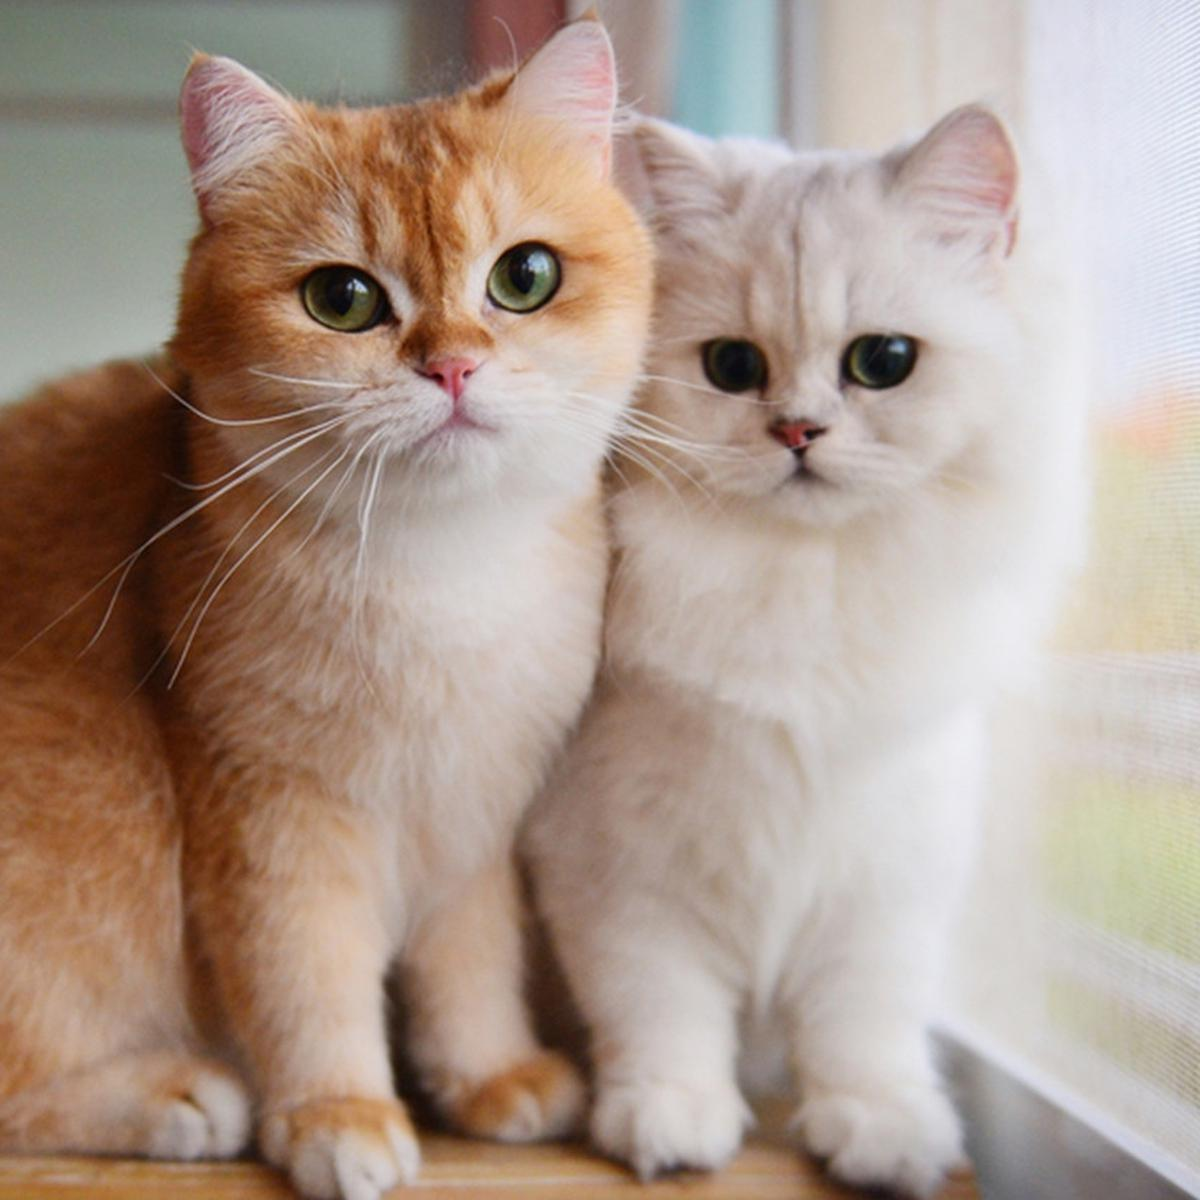
\includegraphics[width=\linewidth]{gambar-kucing.jpg}
        \caption{Kucing Lucu 1}
        \label{fig:kucing-a}
    \end{subfigure}
    \hfill
    \begin{subfigure}[b]{0.3\textwidth}
        \centering
        
\includegraphics[width=\linewidth]{logo-uny.png}
        \caption{Logo UNY}
        \label{fig:logo-uny-b}
    \end{subfigure}
    \hfill
    \begin{subfigure}[b]{0.3\textwidth}
        \centering
        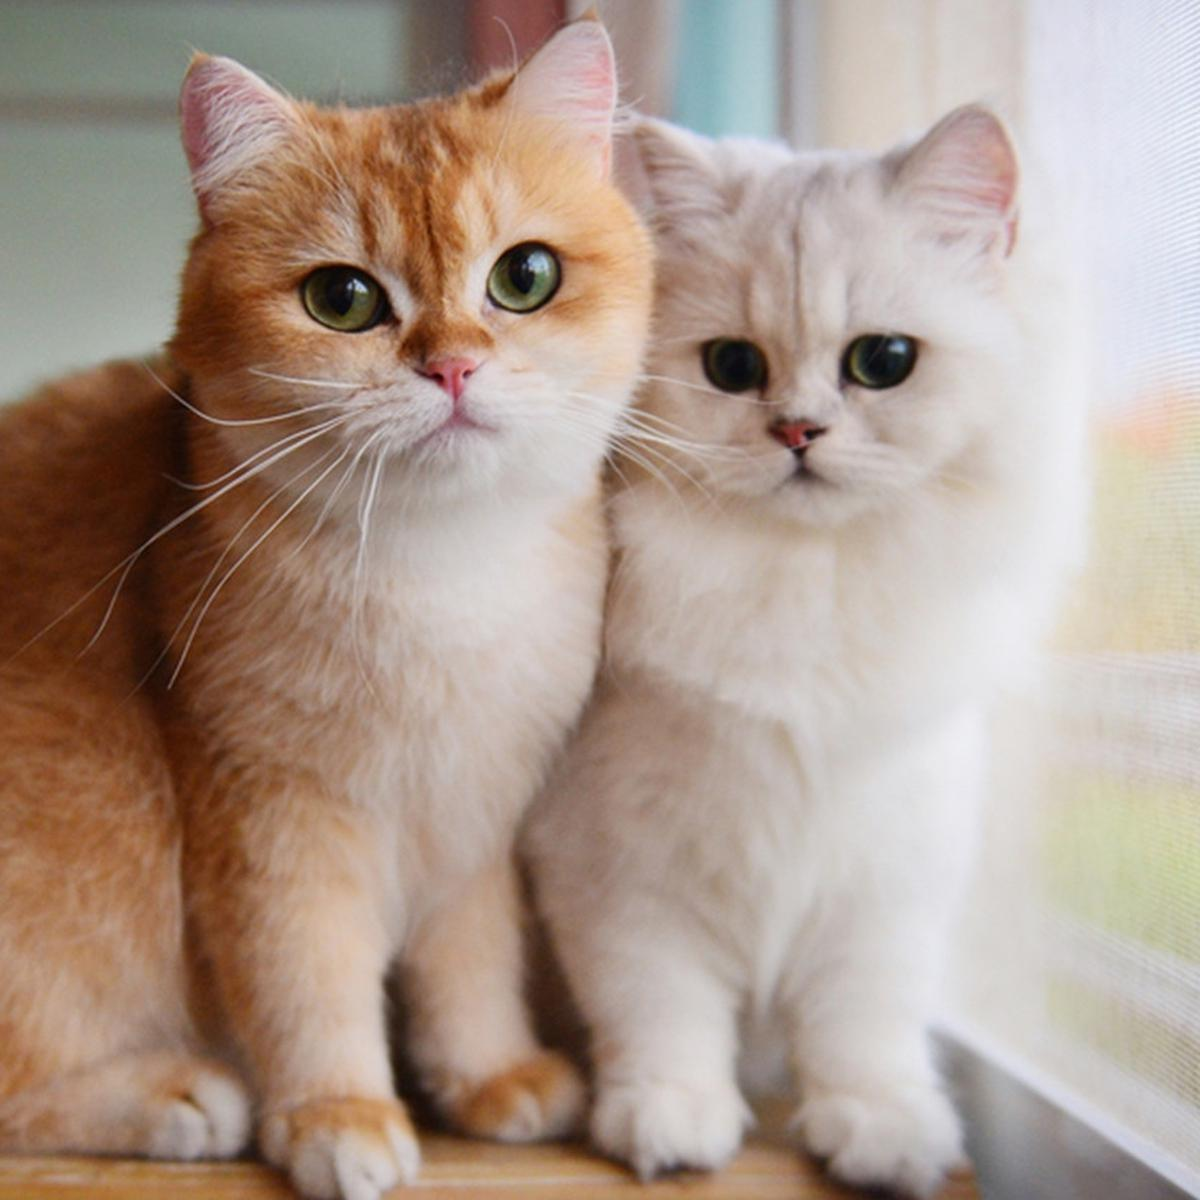
\includegraphics[width=\linewidth]{gambar-kucing.jpg}
        \caption{Kucing Lucu 2}
        \label{fig:kucing-c}
    \end{subfigure}
    \caption{Beberapa gambar yang disusun menjadi 1 bagian dengan penomoran (a), (b), dan (c)}
    \label{fig:kucingdanUNY}
\end{figure}

\subsection{Membuat Tabel}
Pada bagian ini akan dijelaskan bagaimana membuat tabel dalam sebuah dokumen \LaTeX. untuk membuat tabel memang agak sedikit sulit, sehingga saya menyarankan menggunakan tool berikut \url{https://www.tablesgenerator.com/} atau \url{https://www.latex-tables.com/} kemudian isikan tabel pada tool generator tersebut dan salin kodenya ke dalam dokumen \LaTeX. Berikut adalah contoh dari sebuah tabel yang telah dibuat. Jangan lupa setiap tabel harus dimention dan dijelaskan dibacaan seperti berikut ini \cref{tab:hresult}. Contoh pembuatan tabel terlihat kodenya pada \cref{lst:kode_tabel}.

\begin{lstlisting}[language=TeX, caption=Kode untuk Membuat Tabel dalam Dokumen, label=lst:kode_tabel]
    \begin{table}[h]
        \caption{Performance Using Hard Decision Detection}
        \label{tab:hresult}
        \centering
        \begin{tabular}{c rrrrrrr}
            \hline\hline
            Audio Name&\multicolumn{7}{c}{Sum of Extracted Bits} \\ [0.5ex] 
            \hline
            Police & 5 & -1 & 5& 5& -7& -5& 3\\
            Midnight & 7 & -3 & 5& 3& -1& -3& 5\\
            News & 9 & -3 & 7& 9& -5& -1& 9\\[0.8ex]
            \hline
        \end{tabular}
    \end{table}
\end{lstlisting}

\noindent Berikut adalah penjelasan dari setiap bagian kode di atas:

\begin{packed_enum}
    \item \texttt{\textbackslash begin\{table\}[h] ... \textbackslash end\{table\}}: Lingkungan \texttt{table} digunakan untuk membuat tabel dan menempatkannya di posisi tertentu dalam dokumen. Parameter \texttt{[h]} menginstruksikan LaTeX untuk menempatkan tabel di posisi yang paling mendekati lokasi kode tersebut dalam teks. Jika posisi ini tidak berfungsi dengan baik, Anda bisa menggunakan parameter lain, seperti \texttt{[H]} (dari paket \texttt{float}) untuk menempatkan tabel di lokasi yang lebih spesifik.
    \item \texttt{\textbackslash caption\{Performance Using Hard Decision Detection\}}: Menambahkan keterangan (caption) di atas tabel. Caption ini akan otomatis ditampilkan dalam Daftar Tabel dan diberi nomor secara otomatis oleh LaTeX.
    \item \texttt{\textbackslash label\{tab:hresult\}}: Memberi label pada tabel, memungkinkan tabel dirujuk dalam teks menggunakan perintah \texttt{\textbackslash cref\{tab:hresult\}} atau \texttt{\textbackslash ref\{tab:hresult\}}, yang akan menghasilkan "Tabel 1" atau sesuai penomoran tabel.
    \item \texttt{\textbackslash centering}: Mengatur tabel agar berada di tengah halaman.
    \item \texttt{\textbackslash begin\{tabular\}\{c rrrrrrr\} ... \textbackslash end\{tabular\}}: Lingkungan \texttt{tabular} digunakan untuk membuat struktur tabel. Pengaturan kolom menggunakan karakter:
        \begin{packed_enum}
            \item \texttt{c}: Mengatur kolom pertama rata tengah.
            \item \texttt{r}: Mengatur tujuh kolom berikutnya rata kanan.
        \end{packed_enum}
    \item \texttt{\textbackslash hline}: Menambahkan garis horizontal di tabel. Dua \texttt{\textbackslash hline} berturut-turut digunakan untuk garis ganda pada bagian header tabel.
    \item \texttt{\textbackslash multicolumn\{7\}\{c\}\{Sum of Extracted Bits\}}: Menggabungkan tujuh kolom berikutnya menjadi satu sel besar yang berisi teks "Sum of Extracted Bits", yang disejajarkan ke tengah dengan pengaturan \texttt{c}.
    \item Isi tabel, seperti:
        \begin{packed_enum}
            \item \texttt{Police}: Data pada baris ini terkait audio "Police", dengan tujuh angka di kolom berikutnya yang merepresentasikan "Sum of Extracted Bits".
            \item Baris lain mengikuti format yang sama.
        \end{packed_enum}
    \item Jarak tambahan antara baris terakhir dan \texttt{\textbackslash hline} berikutnya diberikan dengan parameter opsional \texttt{[0.8ex]}, yang menambahkan spasi vertikal untuk keterbacaan.
\end{packed_enum}

Dengan penjelasan ini, kode menghasilkan tabel terstruktur yang diberi nomor secara otomatis dan dapat dirujuk di teks dokumen. Hasil tabel dari \cref{lst:kode_tabel} adalah terlihat pada \cref{tab:hresult}.

\begin{table}[h]
    \caption{Performance Using Hard Decision Detection}
    \label{tab:hresult}
    \centering
    \begin{tabular}{c rrrrrrr}
        \hline\hline
        Audio Name&\multicolumn{7}{c}{Sum of Extracted Bits} \\ [0.5ex] 
        \hline
        Police & 5 & -1 & 5& 5& -7& -5& 3\\
        Midnight & 7 & -3 & 5& 3& -1& -3& 5\\
        News & 9 & -3 & 7& 9& -5& -1& 9\\[0.8ex]
        \hline
    \end{tabular}
\end{table}

Kita juga bisa menambahkan tabel yang besar dengan format halaman landscape seperti contoh berikut dan mention tabel seperti berikut ini \cref{tab:LPer} dan berikut ini \cref{tab:PPer}.

\begin{lstlisting}[language=TeX, caption=Kode untuk Membuat Tabel dalam Dokumen dengan Sideway, label=lst:kode_tabel_sideway]
    \begin{sidewaystable}[htbp]
        \caption{Performance After Post Filtering}
        \label{tab:LPer}
        \centering
        \begin{tabular}{l c c rrrrrrr}
            \hline\hline
            Audio &Audibility & Decision &\multicolumn{7}{c}{Sum of Extracted Bits} 
            \\ [0.5ex] 
            \hline
            & &soft &1 & $-1$ & 1 & 1 & $-1$ & $-1$ & 1 \\[-1ex]
            \raisebox{1.5ex}{Police} & \raisebox{1.5ex}{5}&hard
            & 2 & $-4$ & 4 & 4 & $-2$ & $-4$ & 4 \\[1ex]
            & &soft & 1 & $-1$ & 1 & 1 & $-1$ & $-1$ & 1 \\[-1ex]
            \raisebox{1.5ex}{Beethoven} & \raisebox{1.5ex}{5}& hard
            &8 & $-8$ & 2 & 8 & $-8$ & $-8$ & 6 \\[1ex]
            & &soft & 1 & $-1$ & 1 & 1 & $-1$ & $-1$ & 1 \\[-1ex]
            \raisebox{1.5ex}{Metallica} & \raisebox{1.5ex}{5}& hard
            &4 & $-8$ & 8 & 4 & $-8$ & $-8$ & 8 \\[1ex]
            \hline
        \end{tabular}
    \end{sidewaystable}
\end{lstlisting}

\noindent Berikut adalah penjelasan dari setiap bagian kode di atas:

\begin{packed_enum}
    \item \texttt{\textbackslash begin\{sidewaystable\}[htbp] ... \textbackslash end\{sidewaystable\}}: Lingkungan \texttt{sidewaystable} dari paket \texttt{rotating} digunakan untuk menampilkan tabel dalam orientasi landscape. Parameter \texttt{[htbp]} menunjukkan preferensi posisi tabel pada dokumen. Pastikan Anda telah memuat paket \texttt{rotating} di preamble dengan perintah \texttt{\textbackslash usepackage\{rotating\}}.
    \item \texttt{\textbackslash caption\{Performance After Post Filtering\}}: Menambahkan caption (keterangan) di atas tabel. Caption ini akan otomatis dimasukkan dalam Daftar Tabel dan diberi nomor secara otomatis.
    \item \texttt{\textbackslash label\{tab:LPer\}}: Memberi label pada tabel, memungkinkan Anda merujuk tabel ini dalam teks menggunakan perintah \texttt{\textbackslash cref\{tab:LPer\}} atau \texttt{\textbackslash ref\{tab:LPer\}}, yang akan menghasilkan "Tabel 1" atau sesuai penomoran tabel.
    \item \texttt{\textbackslash centering}: Mengatur tabel agar berada di tengah halaman.
    \item \texttt{\textbackslash begin\{tabular\}\{l c c rrrrrrr\} ... \textbackslash end\{tabular\}}: Lingkungan \texttt{tabular} digunakan untuk membuat struktur tabel dengan pengaturan kolom sebagai berikut:
        \begin{packed_enum}
            \item \texttt{l}: Mengatur kolom pertama rata kiri untuk kolom "Audio".
            \item \texttt{c}: Mengatur kolom kedua dan ketiga rata tengah untuk kolom "Audibility" dan "Decision".
            \item \texttt{r}: Tujuh kolom berikutnya rata kanan untuk data "Sum of Extracted Bits".
        \end{packed_enum}
    \item \texttt{\textbackslash hline}: Menambahkan garis horizontal di tabel. Dua \texttt{\textbackslash hline} berturut-turut digunakan untuk garis ganda pada bagian header tabel.
    \item \texttt{\textbackslash multicolumn\{7\}\{c\}\{Sum of Extracted Bits\}}: Menggabungkan tujuh kolom berikutnya menjadi satu sel besar yang berisi teks "Sum of Extracted Bits", yang disejajarkan ke tengah dengan pengaturan \texttt{c}.
    \item Isi tabel, misalnya:
        \begin{packed_enum}
            \item Data pada baris pertama terkait audio "Police", dengan kolom audibility berisi nilai 5, dan data decision dengan dua opsi: "soft" dan "hard".
            \item Data "soft" pada baris pertama dan "hard" pada baris kedua diisi dengan angka sesuai kolom masing-masing.
            \item Untuk beberapa entri seperti "Police", "Beethoven", dan "Metallica", kolom audibility dan audio di tengah (seperti nilai 5) diangkat dengan perintah \texttt{\textbackslash raisebox} untuk memberikan efek centering pada teks.
        \end{packed_enum}
    \item \texttt{[1ex]} atau \texttt{[-1ex]}: Mengatur jarak antar baris untuk menjaga keterbacaan dan posisi elemen tabel yang lebih seimbang.
\end{packed_enum}

Kode ini akan menghasilkan tabel landscape dengan satu caption, beberapa kolom gabungan, dan penomoran otomatis dan hasilnya terlihat pada \cref{tab:LPer}.

\begin{sidewaystable}[htbp]
    \caption{Performance After Post Filtering}
    \label{tab:LPer}
    \centering
    \begin{tabular}{l c c rrrrrrr}
        \hline\hline
        Audio &Audibility & Decision &\multicolumn{7}{c}{Sum of Extracted Bits} 
        \\ [0.5ex] 
        \hline
        & &soft &1 & $-1$ & 1 & 1 & $-1$ & $-1$ & 1 \\[-1ex]
        \raisebox{1.5ex}{Police} & \raisebox{1.5ex}{5}&hard
        & 2 & $-4$ & 4 & 4 & $-2$ & $-4$ & 4 \\[1ex]
        & &soft & 1 & $-1$ & 1 & 1 & $-1$ & $-1$ & 1 \\[-1ex]
        \raisebox{1.5ex}{Beethoven} & \raisebox{1.5ex}{5}& hard
        &8 & $-8$ & 2 & 8 & $-8$ & $-8$ & 6 \\[1ex]
        & &soft & 1 & $-1$ & 1 & 1 & $-1$ & $-1$ & 1 \\[-1ex]
        \raisebox{1.5ex}{Metallica} & \raisebox{1.5ex}{5}& hard
        &4 & $-8$ & 8 & 4 & $-8$ & $-8$ & 8 \\[1ex]
        \hline
    \end{tabular}
\end{sidewaystable}

Contoh lain \cref{lst:kode_tabel_lain} untuk pembuatan tabel seperti di bawah ini dan hasilnya tertampil pada \cref{tab:PPer}.

\begin{lstlisting}[language=TeX, caption=Kode untuk Membuat Tabel dalam Dokumen, label=lst:kode_tabel_lain]
    \begin{table}[ht]
        \caption{Performance After Post Filtering}
        \label{tab:PPer}
        \centering
        \begin{tabular}{l c c rrrrrrr}
            \hline\hline
            Audio &Audibility & Decision &\multicolumn{7}{c}{Sum of Extracted Bits} 
            \\ [0.5ex] 
            \hline
            & &soft &1 & $-1$ & 1 & 1 & $-1$ & $-1$ & 1 \\[-1ex]
            \raisebox{1.5ex}{Police} & \raisebox{1.5ex}{5}&hard
            & 2 & $-4$ & 4 & 4 & $-2$ & $-4$ & 4 \\[1ex]
            & &soft & 1 & $-1$ & 1 & 1 & $-1$ & $-1$ & 1 \\[-1ex]
            \raisebox{1.5ex}{Beethoven} & \raisebox{1.5ex}{5}& hard
            &8 & $-8$ & 2 & 8 & $-8$ & $-8$ & 6 \\[1ex]
            & &soft & 1 & $-1$ & 1 & 1 & $-1$ & $-1$ & 1 \\[-1ex]
            \raisebox{1.5ex}{Metallica} & \raisebox{1.5ex}{5}& hard
            &4 & $-8$ & 8 & 4 & $-8$ & $-8$ & 8 \\[1ex]
            \hline
        \end{tabular}
    \end{table}
\end{lstlisting}

\begin{table}[ht]
	\caption{Performance After Post Filtering}
	\label{tab:PPer}
	\centering
	\begin{tabular}{l c c rrrrrrr}
		\hline\hline
		Audio &Audibility & Decision &\multicolumn{7}{c}{Sum of Extracted Bits} 
		\\ [0.5ex] 
		\hline
		& &soft &1 & $-1$ & 1 & 1 & $-1$ & $-1$ & 1 \\[-1ex]
		\raisebox{1.5ex}{Police} & \raisebox{1.5ex}{5}&hard
		& 2 & $-4$ & 4 & 4 & $-2$ & $-4$ & 4 \\[1ex]
		& &soft & 1 & $-1$ & 1 & 1 & $-1$ & $-1$ & 1 \\[-1ex]
		\raisebox{1.5ex}{Beethoven} & \raisebox{1.5ex}{5}& hard
		&8 & $-8$ & 2 & 8 & $-8$ & $-8$ & 6 \\[1ex]
		& &soft & 1 & $-1$ & 1 & 1 & $-1$ & $-1$ & 1 \\[-1ex]
		\raisebox{1.5ex}{Metallica} & \raisebox{1.5ex}{5}& hard
		&4 & $-8$ & 8 & 4 & $-8$ & $-8$ & 8 \\[1ex]
		\hline
	\end{tabular}
\end{table}

\subsection{Menambahkan Persamaan}

Persamaan tidak lepas dari bidang ilmu teknik dan kadang perlu dituliskan dalam sebuah laporan. Sangat mudah menuliskan persamaan pada sebuah dokumen \LaTeX. Terdapat 2 jenis penulisan persamaan, yaitu inline dengan text seperti contoh ini \(x^2 + y^2 = z^2\) atau seperti ini $E=mc^2$. Jenis lain adalah dituliskan seperti di bawah ini, yang otomatis akan mendapatkan penomoran. Apabila belum familiar dengan kode untuk penulisan persamaan pada \LaTeX, Anda bisa menggunakan tool berikut \url{https://latex.codecogs.com/eqneditor/editor.php} atau \url{https://latexeditor.lagrida.com/}. Setiap persamaan harus disebutkan dalam teks seperti \cref{eq:satu} dan \cref{eq:equationDua} dan dijelaskan terkait persamaan tersebut untuk apa.

\begin{lstlisting}[language=TeX, caption=Kode untuk Menulis Persamaan, label=lst:kode_persamaan_emc]
    \begin{equation}
        \label{eq:satu}
        E=mc^2
    \end{equation}
\end{lstlisting}

\begin{lstlisting}[language=TeX, caption=Kode untuk Menulis Persamaan, label=lst:kode_persamaan_mn]
    \begin{equation}
        \label{eq:equationDua}
        m_n = k_p*e_n + \frac{k_e*T}{T_{reset}}\sum_{i=0}^{n}e_i + k_d\frac{e_n - e_{n-1}}{\delta t} + m_{R}
    \end{equation}
\end{lstlisting}

\noindent Berikut adalah penjelasan dari setiap bagian kode di atas:

Dengan menggunakan lingkungan \texttt{equation}, Anda bisa menulis dan memberi nomor persamaan secara otomatis serta merujuknya dengan mudah dalam teks menggunakan \texttt{\textbackslash cref}.

\begin{equation}
    \label{eq:satu}
    E=mc^2
\end{equation}

\begin{equation}
    \label{eq:equationDua}
    m_n = k_p*e_n + \frac{k_e*T}{T_{reset}}\sum_{i=0}^{n}e_i + k_d\frac{e_n - e_{n-1}}{\delta t} + m_{R}
\end{equation}

\subsection{Referensi dan Sitasi}
Referensi dan sitasi pada dokumen \LaTeX juga cukup mudah. Silahkan buka file \textit{pustaka.bib} dan amati beberapa contoh penulisan referensi yang ada. Untuk menggenerate bentuk referensi seperti ini dapat menggunakan Mendeley atau Zotero. Mensitasi referensi seperti ini \citep{Priambodo_2021}, \citep{Nasuha_2017}, \citep{Dhewa_Dharmawan_Priyambodo_2017}, \citep{Arifin_2015} dapat dilakukan dengan perintah \verb|\citep{nama_label}|. Pemberian sitasi dengan benar membuat sitasi tersebut dapat di klik dan akan mengarahkan ke daftar pustaka.